\documentclass[tikz,border=10pt]{standalone}
\usetikzlibrary{calc}

\begin{document}
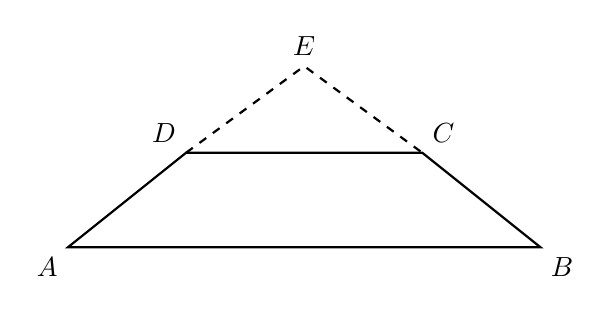
\begin{tikzpicture}[>=stealth, thick]

    % 1. 定义坐标点
    % 设底边 AB 在 x 轴上，对称分布
    \coordinate (A) at (0,0);
    \coordinate (B) at (6,0);
    \coordinate (D) at (1.5,1.2);
    \coordinate (C) at (4.5,1.2);
    \coordinate (E) at (3,2.3); % 顶部顶点

    % 2. 绘制梯形实线部分 ABCD
    \draw (A) -- (B) -- (C) -- (D) -- cycle;

    % 3. 绘制缺失的三角形顶边虚线部分 EC 和 ED
    \draw[dashed] (D) -- (E) -- (C);

    % 4. 标注点位
    \node[below left] at (A) {$A$};
    \node[below right] at (B) {$B$};
    \node[above right] at (C) {$C$};
    \node[above left] at (D) {$D$};
    \node[above] at (E) {$E$};

\end{tikzpicture}
\end{document}